\documentclass[10pt,a4paper]{article}

%% PACCHETTI AGGIUNTIVI
\usepackage{amssymb,amsmath,amsthm,amsfonts}
%\usepackage{bm}
\usepackage{calc}
%\usepackage[inline]{enumitem}
%\usepackage{ifthen}
%\usepackage[utf8]{inputenc}
\usepackage[portrait]{geometry}
\usepackage{graphicx}
%\usepackage[colorlinks=true,citecolor=blue,linkcolor=blue]{hyperref}
\usepackage{mathrsfs}
\usepackage{multicol,multirow}
%\usepackage{subcaption}
%\usepackage{tabularx}
%\usepackage[absolute]{textpos}
%\usepackage{titlesec}
%\usepackage{wrapfig}
%\usepackage{xfrac}

%% GEOMETRIA
\geometry{top=1cm,bottom=1cm,left=.7cm,right=.7cm}

%%	STILE
\pagestyle{empty}
\raggedright

%%	HEADINGS
%%	Numerazione
\setcounter{secnumdepth}{0}
\setlength{\parindent}{3pt}
\setlength{\parskip}{0pt plus 0.5ex}
%%	Formattazione
\makeatletter
\renewcommand{\section}{\@startsection{section}{1}
	{0mm}{2ex}{.1ex}{\normalfont\large\bfseries}}
\renewcommand{\subsection}{\@startsection{subsection}{2}
	{0mm}{.5ex}{.1ex}{\normalfont\normalsize\bfseries}}
\renewcommand{\subsubsection}{\@startsection{subsubsection}{3}
	{0mm}{.1ex}{.1ex}{\normalfont\small\bfseries}}
\makeatother

%%	DEFINIZIONE COMANDI
\newcommand{\de}{\mathrm d}
\newcommand{\fracd}[2]{\frac{\de #1}{\de #2}}
\newcommand{\fracp}[2]{\frac{\partial #1}{\partial #2}}
\newcommand{\fracpq}[2]{\frac{\partial^2 #1}{{\partial #2}^2}}
\newcommand{\fracpp}[3]{\frac{\partial^2 #1}{\partial #2 \partial #3}}
\newcommand{\grad}[1]{\text{grad}\,#1}
\newcommand{\dive}[1]{\text{div}\,#1}
\newcommand{\rot}[1]{\text{rot}\,#1}
\newcommand{\vers}{\mathop{\text{vers}}}
\newcommand{\itemm}[1]{\indent - #1\\}



\begin{document}
	
\raggedright

\begin{multicols}{2}
	
	\section{ELETTROSTATICA NEL VUOTO}
\subsection{Legge di Coulomb, campo e potenziale elettrostatico}
$\mathbf F_{2\to1}(\mathbf r_2-\mathbf r_1)=q_2\mathbf E_1(\mathbf r_2)=\frac{q_1q_2}{4\pi\varepsilon_0} \frac{\mathbf r_1-\mathbf r_2}{|\mathbf r_1-\mathbf r_2|^3} = \frac{q_1q_2}{4\pi\varepsilon_0} \frac{\vers(\mathbf r_1-\mathbf r_2)}{|\mathbf r_1-\mathbf r_2|^2}$
$\mathbf E(\mathbf r) = \frac1{4\pi\varepsilon_0} \left[ \int_\Upsilon \frac{\varrho(\mathbf r^\prime)(\mathbf r-\mathbf r^\prime)}{| \mathbf r-\mathbf r ^\prime|^3} \de\upsilon^\prime + \sum_{i=1}^N \frac{q_i(\mathbf r-\mathbf r_i)}{|\mathbf r-\mathbf r_i|^3} \right]$
$V(\mathbf r) = \frac1{4\pi\varepsilon_0} \left[ \int_\Upsilon \frac{\varrho(\mathbf r^\prime)}{|\mathbf r-\mathbf r^\prime|} \de\upsilon^\prime + \sum_{i=1}^N\frac{q_i}{|\mathbf r-\mathbf r_i|}\right]$

\subsection{Teorema di Gauss e I equazione di Maxwell}
$\Phi_{\partial \mathcal G}(\mathbf E) = \frac1{\varepsilon_0} \int_\mathcal G \varrho(\mathbf r^\prime) \, d\upsilon'\;\;\Rightarrow\;\;\dive\,\mathbf E=\frac \varrho{\varepsilon_0}$

\subsection{Equazione di Poisson e di Laplace}
$\mathbf E=-\vec\nabla V\;\Rightarrow\;
\nabla^2V(\mathbf r)=\frac {\varrho(\mathbf r)}{\varepsilon_0}\qquad
\rho(\mathbf r)\equiv 0\;\Rightarrow\;\nabla^2V(\mathbf r)=0$

%\subsection{Alcune costanti dielettriche}
%$\varepsilon_0_0=8.854\cdot 10^{-12}\:\mathrm{\frac{C^2}{N\,m^2}}$\\
%\begin{tabular}{@{}l|c}\;\;Materiale&$\varepsilon_0_r$\\
%\hline
%aria a 25$^\circ$&1.0005\\
%acqua a 25$^\circ$&78\\
%gomma&3\\
%porcellana&6\\
%carta paraffinata&2\\
%vetro&4\,$\div$\,10\\
%\end{tabular}\\

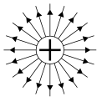
\includegraphics[bb=0 0 100 100]{positiva.png}\qquad
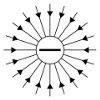
\includegraphics[bb=0 0 100 100]{negativa.png}

	\section{MAGNETOSTATICA NEL VUOTO}
\subsection{Campo di induzione generato da cariche in moto}
\begin{tabular}{@{}ll}
conduttore filiforme&conduttore generico\\
$\de\mathbf B(\mathbf r) = \frac{\mu_0}{4\pi} \frac{i\mathrm \de\mathbf r^\prime \times (\mathbf r-\mathbf r^\prime)}{|\mathbf r-\mathbf r^\prime|^3}$&
$\de\mathbf B(\mathbf r) = \frac{\mu_0}{4\pi} \frac{\mathbf J(\mathbf r^\prime) \de\upsilon^\prime \times (\mathbf r-\mathbf r^\prime)}{|\mathbf r-\mathbf r^\prime|^3}$
\end{tabular}

\subsection{II equazione di Maxwell e potenziale magnetico}
$\Phi_{\partial\mathcal G}(\mathbf B) = 0 \;\Rightarrow\; \dive\mathbf B = 0 \;\Rightarrow\; \mathbf B = \rot\mathbf A$

\subsection{Teorema di Ampère e IV equazione di Maxwell}
$\oint_\gamma \mathbf B \cdot \de\mathbf s = \mu_0 \sum_k m_k i_k \;\;\Rightarrow\;\; \rot\mathbf B = \mu_0\mathbf J$\\
$m_i$ - grado di concatenazione di $I_i$

\subsection{Equazione di Poisson}
$\mathbf B = \rot\mathbf A \;\Rightarrow\; \rot\mathbf B = $

\subsection{Legge di Ampère per campo di induzione magnetica}
\begin{tabular}{@{}ll}
	conduttore filiforme&conduttore generico\\
	$\de\mathbf F = i\mathrm d\mathbf l \times \mathbf B$ & $\de\mathbf F = \mathbf J\de\upsilon \times \mathbf B$\\
	$\de\mathbf M = \mathbf r \times (i\mathrm \de\mathbf l \times \mathbf B)$ & $\de\mathbf M = \mathbf r \times (\mathbf J\de\upsilon \times \mathbf B)$\end{tabular}

	\section{ASPETTI ENERGETICI}
\subsection{Lavoro, potenziale, energia elettrostatica}
$L_{AB} = \int_A^B \mathbf F \cdot \de\mathbf s = q \int_A^B \mathbf E \cdot \de\mathbf s = -q \int_A^B \vec\nabla V \cdot \de\mathbf s = -q \int_A^B \de V$\\
$V_O(P) = -\int_O^P \mathbf E \cdot \de\mathbf s$\\
$L_{AB} = -q \Delta V = \Delta U \;\;\Longrightarrow\;\; U = -qV$\\

\subsection{Conservatività e III equaz. di Maxwell stazionaria}	
$\oint \mathbf E \cdot \de\mathbf s = 0 \;\;\Rightarrow\;\; \rot\mathbf E = 0$

%\subsection{sistemi di cariche discrete}
%\begin{tabular}{@{}lll}
%una carica&due cariche&$n$ cariche\\
%$U(\mathbf r)=q\,V(\mathbf r)$&$U=\frac{q_1q_2}{4\pi\varepsilon}\frac{1}{r_{12}}$&$U=\frac 12\underset{i\neq j}{\sum}\frac{1}{4\pi\varepsilon}\frac{q_iq_j}{r_{ij}}=\frac 12\sum_i q_iV_i$\end{tabular}\\
%$V_i=\sum_j \frac{q_j}{4\pi\varepsilon r_{ij}}$ potenziale generato in $P_i$ dalle altre cariche
%
%$\Delta T = L_{AB} \Rightarrow \frac12 m(v_B^2-v_A^2) = q(V_A - V_B)$

%\subsection{Sistema di cariche distribuite}
%$U=\frac 12 \int_\Upsilon\varrho V\,\de\upsilon=\frac \varepsilon 2 \int_\Upsilon V\,\dive\mathbf E\,\de\upsilon=\frac \varepsilon 2\int_\Upsilon[\dive(V\mathbf E)+\|\mathbf E\|^2]\,\de\upsilon=$\\$\!\!\!=\frac \varepsilon 2\int_{\partial\Upsilon}V\,\mathbf E\cdot\mathbf n\,\de S+\frac \varepsilon 2\int_\Upsilon \|\mathbf E\|^2\,\de\upsilon\quad\underset{\Upsilon\to\mathbb{E}^3}{\lim}U=\int_{\mathbb{E}^3}\!\frac{\varepsilon \|\mathbf E\|^2}{2}\,\de\upsilon=\int_{\mathbb{E}^3}\!u\,\de\upsilon$

%\subsection{Carica in moto in un campo di induzione uniforme}
%\subsubsection{Ipotesi}
%$\mathbf B_0=B\mathbf u\qquad\|\mathbf v(t)\|=v_0\qquad\mathbf v_0=\mathbf v_0^\parallel+\mathbf v_0^\perp\qquad\mathbf v_0^\parallel=\mathbf v_0\cdot\mathbf u=v_0\cos\theta$\\
%\subsubsection{Equazione del moto}
%$qB\mathbf v_0^\perp\times\mathbf u=m\vec a\;\;\Rightarrow\;\begin{cases}\vec a^\parallel=\vec 0\\\frac{v_0^2}{r}=\frac{qBv_0\sin\theta}{m}\end{cases}\!\!\!\!\Rightarrow\;\begin{cases}\mathbf v^\parallel=v_0\cos\theta\,\mathbf u\\\omega=\frac{qB}{m}\quad r=\frac{mv_0\sin\theta}{qB}\end{cases}$\\
%moto elicoidale cilindrico di passo $p=v_0^\parallel\,T=\frac{2\pi m v_0\sin\theta}{qB}$

%	\section{ELETTROMAGNETISMO NON STAZIONARIO}
%\subsection{Legge di F-N-L e III equaz. di Maxwell}
%$f_\mathrm{ind}=-\frac{\de\Phi_\gamma(\mathbf B)}{\de t}\qquad f_\mathrm{ind}=\oint_\gamma\mathbf E_\mathrm{ind}\cdot\de \mathbf s\quad \mathbf E_\mathrm{ind}=\mathbf E+\mathbf v_\mathrm{tr}\times\mathbf B$\\
%se $\mathbf v_\mathrm{tr}=\vec 0$ (circuito fermo) allora $\rot\,\mathbf E=-\frac{\partial\mathbf B}{\partial t}$
%\subsection{IV equazione di Maxwell}
%\subsection{Coeff. di mutua induzione}
%$M_{21}=\frac{\Phi_1(\mathbf B_2)}{I_2}\;\Rightarrow\;f_\text{ind}=-M_{21}\frac{\de I_1}{\de t}\qquad M_{21}=M_{12}$
%\subsection{Autoinduzione}
%\subsubsection{flusso concatenato, induttanza e f.e.m. autoindotta}
%$\Phi_\gamma(\mathbf B_0)=I\Big(\frac{\mu_0}{4\pi}\int_{\Sigma(\gamma)}\oint_\gamma\frac{\de\mathbf l\times\Delta\mathbf r}{\|\Delta\mathbf r\|^3}\cdot\mathbf n\,\de\mathbf s\Big)\qquad L=\frac{\Phi_\gamma(\mathbf B_0)}{I}\qquad f_\mathrm a=-L\frac{\de I}{\de t}$
%\subsubsection{energia immagazzinata in un induttore}
%incremento dovuto al passaggio di corrente\quad$\de U=LI\,\de I$\\
%energia di un induttore carico\quad$U=\frac 12 LI^2$

\vfill\null\columnbreak

	\section{DIELETTRICI}
\subsection{Cariche e correnti di polarizzazione}
$\begin{array}{l} \langle\mathbf p\rangle = \frac{\sum_i \mathbf p_i}{n\Delta V}\\
	\mathbf P = n\langle\mathbf p\rangle\end{array}
\begin{array}{l} \sigma_{pol} = \mathbf P \cdot \mathbf n \\
	\rho_{pol} = -\dive\mathbf P\end{array}
\begin{array}{l} \mathbf J_{pol} = \fracp{}{t}\{nq(\mathbf r_+ - \mathbf r_-)\} = \fracp{\mathbf P}{t} \\
	\dive\mathbf J_{pol} + \fracp{\rho_{pol}}{t}=0\end{array}$

\subsection{Contributi a campo e potenziale}
$V_{pol}(\mathbf r) = \frac1{4\pi\varepsilon_0} \int_S \frac{\mathbf P \cdot \mathbf n}{|\mathbf r - \mathbf r^\prime|} \de\varsigma^\prime - \int_V \frac{\dive\mathbf P}{|\mathbf r - \mathbf r^\prime|} \de\upsilon^\prime \qquad \mathbf E_{pol} = -\nabla V_{pol}$\\
$\mathbf E = \mathbf E_{lib} + \mathbf E_{pol} \qquad V = V_{lib} + V_{pol}$

\subsection{I equazione di Maxwell per dielettrici}
$\dive\mathbf D = \rho_{lib} \qquad \mathbf D = \varepsilon_0\mathbf E + \mathbf P$

\subsection{Costanti del dielettrico}
$\langle\mathbf p\rangle = \alpha \varepsilon_0\mathbf E \qquad \mathbf P = \chi_e \varepsilon_0\mathbf E \qquad \mathbf D = \varepsilon\mathbf E \qquad \varepsilon = \varepsilon_0(1+\chi_e)$

%	\section{CONDUTTORI}
%\subsection{Conduttore isolato}
%$C=\frac{Q}{V}$\quad dipende solo dalla geometria del conduttore\\
%$Q$ e $V$ sono determinati dalla distribuzione di carica
%
%\subsection{Due conduttori}
%$C=\frac{Q}{V_1-V_2}=\frac{-Q}{V_2-V_1}$
%
%\subsection{Collegamento di condensatori}
%in serie $C_\text{eq}=\sum_i C_i$\qquad in parallelo $C_\text{eq}=(\sum_i \frac{1}{C_i})^{-1}$
%
%\subsection{Energia immagazzinata in un condensatore}
%incremento dovuto a traferimento di carica\quad$\de U=\frac{q}{C}\de q$\\
%energia di un condensatore carico\quad$U=\frac 12\frac{Q^2}{C}=\frac 12 QV^2$
%
%	\section{CORRENTI ELETTRICHE STAZIONARIE}
%\subsection{Densità di corrente e corrente elettrica}
%$\mathbf J = n q \mathbf v_{der}=\varrho\,\mathbf v_{der} \quad \mathbf v_{der} \parallel \mathbf E \qquad \de q = n q \mathbf v_{der} \de t \cdot \mathbf n \de S$\\
%$\de i = \frac{\de q}{\de t} = \mathbf J \cdot \mathbf n \de S \;\;\Rightarrow\;\; i(\Sigma) = \int_\Sigma \mathbf J \cdot \mathbf n \de S$
%
%\subsection{Legge di Ohm}
%$\mathbf J = \tilde\sigma \mathbf E$\qquad per mezzi isotropi $\tilde\sigma = \sigma\tilde I \;\Rightarrow\; \mathbf J = \sigma\mathbf E \;\Rightarrow\; \mathbf E = \rho\mathbf J$
%
%\subsection{Conservazione della carica e I legge di Kirchhoff}
%$\frac{\de}{\de t} \int_\Upsilon \varrho \de\upsilon = \int_{\partial\Upsilon} \mathbf J \cdot (-\mathbf n) \de S \qquad \frac{\partial\varrho}{\partial t} + \dive\mathbf J = 0$\\
%per un nodo di $n$ conduttori \quad $\sum_k^{(alg)} i_k=0$
%
%\subsection{Circuitazione campo elettrico e II legge di Kirchhoff}
%$\mathbf E = \mathbf E^\mathrm s + \mathbf E^\mathrm m + \mathbf E^\mathrm c = \rho\mathbf J \;\;\Rightarrow\;\; \sum_i^{(alg)} {\mathcal E_i}^\mathrm m + \sum_i^{(alg)} {\mathcal E_i}^\mathrm c = i R_{tot}$ 	
%
%\subsection{Resistività}
%$R(T) = \rho(T) \frac LS \qquad \rho(T) = \rho_0 (1+\alpha T)$

\vfill\null
\end{multicols}

\newpage
\footnotesize

\begin{multicols}{2}
\setlength{\premulticols}{1pt}
\setlength{\postmulticols}{1pt}
\setlength{\multicolsep}{1pt}
\setlength{\columnsep}{2pt}

	\section{CALCOLO CAMPO ELETTROSTATICO}
\subsection{Dipolo elettrico}
$\varrho = \{(Q,\frac D 2\mathbf u),(-Q,-\frac D 2\mathbf u)\} \:\Rightarrow\: \begin{array}{l}
	\mathbf E(d \mathbf u) = -\frac{Q}{4\pi\varepsilon} \frac D{(d^2+\frac{D^2}{4})^{3/2}} \mathbf k\\
	V(d \mathbf u) = \end{array}$

\subsection{Filo rettilineo indefinito}
$\varrho=\lambda_0\;\Rightarrow\;\begin{array}{@{}l}
\mathbf E(r\mathbf u_r)=\frac{\lambda_0}{2\pi\varepsilon}\frac 1 r\mathbf u_r\\
V(r\mathbf u_r)=\frac{\lambda_0}{2\pi\varepsilon}\log r\end{array}$\\
$I= I_0\;\Rightarrow\;
\mathbf B_0(r\mathbf u_r)=\frac{\mu_0 I_0}{2\pi}\frac 1 r \mathbf u_\theta$

\subsection{Spira circolare}
$\varrho=\lambda_0\;\Rightarrow\;\begin{array}{@{}l}
\mathbf E(z\mathbf u_z)=\frac{\lambda_0 R}{2\varepsilon}\frac {z}{(z^2+R^2)^{3/2}}\mathbf u_z\\
V(z\mathbf u_z)=\frac{\lambda_0 R}{2\varepsilon}\frac{1}{\sqrt{z^2+R^2}}\end{array}$\\
$I= I_0\;\Rightarrow\;\mathbf B_0(z\mathbf u_z)=\frac{\mu_0I_0}{2}\frac{R^2}{(z^2+R^2)^{3/2}}\mathbf u_z=\frac{\mu_0}{2\pi}\frac{\mathbf M}{(z^2+R^2)^{3/2}}$

\subsection{Corona circolare}
$\varrho=\sigma_0\:\Rightarrow\:\begin{array}{l}
\mathbf E(z\mathbf u_z)=\frac{\sigma_0 z}{2\varepsilon}(\frac{1}{\sqrt{{R_\mathrm{i}}^2+z^2}}-\frac1{\sqrt{{R_\mathrm{e}}^2+z^2}})\mathbf u_z\\
V(z\mathbf u_z)=\frac{\sigma_0}{2\varepsilon}(\sqrt{z^2+R_\mathrm{i}^2}-\sqrt{z^2+R_\mathrm{e}^2})\end{array}$

\subsection{Disco}
$\varrho=\sigma_0\:\Rightarrow\:\begin{array}{l}
\mathbf E(z\mathbf u_z)=\frac{\sigma_0}{2\varepsilon_0}(1-\frac z{\sqrt{z^2+R^2}})\mathbf u_z\\
V(z\mathbf u_z)=\frac{\sigma_0}{2\varepsilon}(\sqrt{z^2+R^2}-z)\end{array}$

\subsection{Piano indefinito}
$\varrho=\sigma_0\:\Rightarrow\:\begin{array}{l}
\mathbf E(x\mathbf n)=\frac{\sigma_0}{2\varepsilon_0}\,\mathbf n\\
V(x\mathbf n)=-\frac{\sigma_0}{2\varepsilon_0}x\end{array}$

\subsection{Doppio piano indefinito}
$\varrho=\sigma_0\:\Rightarrow\:
\mathbf E(x\mathbf n)=\begin{cases}\frac{\sigma_0}{\varepsilon_0}\mathbf n & |x|<\frac D2\\0 & |x|>\frac D2\end{cases}\qquad
V(x\mathbf n)=\begin{cases}-\frac{\sigma_0}{\varepsilon_0}x & |x|<\frac D2\\0 & |x|>\frac D2\end{cases}$

\subsection{Sfera piena}
$\varrho=\begin{cases}
\varrho_0&\!\!r\leq R\\
0&\!\!r>R
\end{cases}\;
\Longrightarrow\;\begin{array}{@{}l}
\mathbf E(r\mathbf u_r)=\begin{cases}
\frac{\varrho}{3\varepsilon_0}r\mathbf u_r=\frac{Q}{4\pi\varepsilon_0 R^3}r\,\mathbf u_r&\!\!r<R\\
\frac{Q}{4\pi\varepsilon_0}\frac1{r^2}\,\mathbf u_r=\frac{\varrho}{3\varepsilon_0}\frac{R^3}{r^2}\mathbf u_r&\!\!r>R\end{cases}\\
V(r)=\begin{cases}
\frac{\varrho_0}{6\varepsilon_0}(R^2-r^2)=\frac{Q}{8\pi\varepsilon_0 R^3}(R^2-r^2)\\
-\frac{Q}{2\pi\varepsilon_0}\frac 1r=-\frac{2\varrho}{3\varepsilon_0}\frac{R^3}{r}\end{cases}
\end{array}$\\
$\varrho=\begin{cases}
\varrho(r\mathbf u_r)&r\leq R\\
0&r>R
\end{cases}\;\;
\Longrightarrow\;\;
\mathbf E(r\mathbf u_r)=\begin{cases}
???&r<R\\
\frac1{4\pi\varepsilon_0}\frac{Q(r)}{r^2}&r>R
\end{cases}$

\subsection{Guscio sferico}
$\varrho=\begin{cases}
\sigma_0&r=R\\
0&r\neq R
\end{cases}\Longrightarrow\;\begin{array}{@{}l}
\mathbf E(r\mathbf u_r)=\begin{cases}
0&r<R\\
\frac{Q}{4\pi\varepsilon_0}\frac{1}{r^2}=\frac{\sigma_0}{\varepsilon_0}\frac{R^2}{r^2}&r>R\end{cases}\\
V(r\mathbf u_r)=\begin{cases}
0&r<R\\
\frac{Q}{4\pi\varepsilon_0}\frac 1r=\frac{\sigma_0}{\varepsilon_0}\frac{R^2}{r}&r>R\end{cases}\end{array}$

\subsection{Corona sferica}
$\varrho=\begin{cases}
\varrho_0&r\in [R_\mathrm{i},R_\mathrm{e}]\\
0&r\not\in [R_\mathrm{i},R_\mathrm{e}]
\end{cases}\;\Longrightarrow\;\begin{array}{@{}l}
\mathbf E(r\mathbf u_r)=\begin{cases}
0&r<R_\mathrm i\\
\frac{\varrho_0}{3\varepsilon_0}\frac{R_\mathrm e^3-R_\mathrm i^3}{r^2}&r\in[R_\mathrm{i},R_\mathrm{e}]\\
\frac{Q}{4\pi\varepsilon_0}\frac{1}{r^2}&r>R_\mathrm e\end{cases}\\
V(r\mathbf u_r)=\begin{cases}
0&r<R_\mathrm i\\
\frac{\varrho_0}{3\varepsilon_0}\frac{R_\mathrm e^3-R_\mathrm i^3}{r}&r\in[R_\mathrm{i},R_\mathrm{e}]\\
\frac{Q}{4\pi\varepsilon_0}\frac 1r&r>R_\mathrm e\end{cases}\end{array}$

\subsection{Cilindro pieno indefinito}
$\varrho=\begin{cases}
\varrho_0&\rho\leq R\\
0&\rho>R
\end{cases}\;\;
\Longrightarrow\;\;\mathbf E(\rho\mathbf u_\rho)=\begin{cases}
\frac{\varrho_0}{2\varepsilon_0}\rho\,\mathbf u_\rho&\rho\leq R\\
\frac{\varrho_0 R^2}{2\varepsilon_0}\frac 1\rho\,\mathbf u_\rho&\rho\geq R
\end{cases}$

\subsection{Guscio cilindrico indefinito}
$\varrho=\begin{cases}
\sigma_0&\rho=R\\
0&\rho\neq R
\end{cases}\;\;
\Longrightarrow\;\;
\mathbf E(\rho\mathbf u_\rho)=\begin{cases}
???&\rho\\
???&\rho
\end{cases}$

\vfill\null
\columnbreak

	\section{CALCOLO CAMPO MAGNETOSTATICO}
\subsection{Spira circolare}

\subsection{Conduttore cilindrico indefinito}
$\mathbf B_0(\rho\mathbf u_\rho)=\begin{cases}\frac{\mu_0I_0}{2\pi R^2}r&\rho<R\\\frac{\mu_0I_0}{2\pi}\frac 1\rho\mathbf u_\theta&\rho\geq R\end{cases}$

\subsection{Nastro rettilineo indefinito}
$\mathbf B_0(d)=\begin{cases}-\frac{\mu_0I_0}{2\pi}\log(\frac{d+L}{L})\mathbf k&d>\frac L2\\\frac{\mu_0I_0}{2\pi}\log(\frac{d+L}{L})\mathbf k&d<-\frac L2\end{cases}$

\subsection{Solenoide cilindrico}
$\mathbf B_0(z\mathbf u_z)=\frac{n\mu_0I_0}{2}(\cos\theta_1-\cos\theta_2)\mathbf u_zs$\\
se $R\ll L$ allora $\begin{array}{l}\theta_1\to 0\\\theta_2\to\pi\end{array}\;\Rightarrow\;\mathbf B_0=\frac{N\mu_0I_0}{L}\mathbf u_z$\\
$\Phi_\mathrm a(\mathbf B_0)=\pi R^2B_0\;\Rightarrow\; L=\frac{N^2\mu_o\pi R^2}{L}$\\
due solenoidi accoppiati\quad$M_{12}=\sqrt{L_1L_2}=\frac{\mu_0N_1N_2S}{L}$

\subsection{Solenoide toroidale}
$B=\frac{\mu_0NI_0}{2\pi r}$
	
	\section{CALCOLO CAPACITÀ}
\subsection{Condensatore piano}
$E(x)=\frac{Q}{\varepsilon_0 S}\quad
\Delta V=\frac{Qd}{\varepsilon_0 S}\;\;
\Longrightarrow\;\;
C=\varepsilon_0\frac{S}{d}$

\subsection{Condensatore sferico}
$E_r(r)=\frac{Q}{4\pi\varepsilon_0}\frac 1r\quad
\Delta V=-\int_{R_\mathrm{i}}^{R_\mathrm{e}}\mathbf E\cdot\de \mathbf s=\frac{Q}{4\pi\varepsilon_0}\frac{R_\mathrm{e}-R_\mathrm{i}}{R_\mathrm{e}R_\mathrm{i}}\;\;
\Longrightarrow\;\;
C=4\pi\varepsilon_0\frac{R_\mathrm{e}R_\mathrm{i}}{R_\mathrm{e}-R_\mathrm{i}}$\\
se $R_\mathrm{i},R_\mathrm{e}\ll (R_\mathrm{e}-R_\mathrm{i})$ allora $C\simeq\varepsilon_0\frac{S_\mathrm{i}}{R_\mathrm{e}-R_\mathrm{i}}$

\subsection{Condensatore cilindrico}
$E_\rho(\rho)=???$

	\section{CIRCUITI CON CORRENTI ALTERNATE}
\subsection{Carica del condensatore}
\itemm{carica sulle armature \quad}
\itemm{d.d.p tra le armature \quad}
\itemm{corrente circolante \quad $i(t)=\frac{\de q(t)}{\de t}=\frac{\mathcal E}{R}e^{-\frac{t}{RC}}$}
\itemm{d.d.p alla resistenza \quad $v_R(t)=i(t)R=\mathcal Ee^{-\frac{t}{RC}}$}
\itemm{potenza del generatore \quad $P_{gen}(t)=\mathcal Ei(t)=\frac{\mathcal E^2}{R}e^{-\frac{t}{RC}}$}
\itemm{potenza sulla resistenza \quad $P_R(t)=Ri^2(t)=\frac{\mathcal E^2}{R}e^{-\frac{2t}{RC}}$}
\itemm{potenza sul condensatore \quad $P_C(t)=v_C(t)i(t)=P_{gen}-P_R$}

\subsection{Scarica del condensatore}

\subsubsection{RC serie}
\itemm{equazione di maglia\quad$\mathcal E-\frac{q(t)}{C}=\frac{\de q(t)}{\de t}R$}
\itemm{carica sulle armature\quad$q(t)=C\mathcal E(1-e^{-\frac{t}{RC}})$}
\itemm{d.d.p. tra le armature\quad$v_C(t)\frac{q(t)}{C}=\mathcal E(1-e^-{t}{RC})$}

\subsubsection{RC parallelo}

\subsection{RL serie}
\itemm{equazione di maglia\quad$\mathcal E-L\frac{\de I}{\de t}=RI$}

\subsection{RL parallelo}

\subsection{LC serie}

\subsection{LC parallelo}

\subsection{RLC serie}

\subsection{RLC parallelo}

\end{multicols}

\end{document}
